\documentclass{jlreq}

\usepackage{bm}
\usepackage{fancyhdr}
\usepackage{float}
\usepackage{graphicx}
\usepackage{listings}

\lstset{
    language=C, % 使用するプログラム言語を指定
    basicstyle=\ttfamily\footnotesize, % フォントの指定
    numbers=left, % 行番号を表示(必要な場合)
    numberstyle=\tiny, % 行番号のスタイル
    frame=single, % ソースコードを枠で囲む(必要な場合)
    breaklines=true, % 長い行を自動的に折り返す
    captionpos=b, % キャプションの位置を下にする
    showstringspaces=false, % 文字列内のスペースを表示しない
    keywordstyle=\color{blue}, % キーワードの色
    commentstyle=\color{green}, % コメントの色
    stringstyle=\color{red}, % 文字列の色
}
\renewcommand{\lstlistingname}{ソースコード}

\pagestyle{fancy}
\fancyhf{}
\fancyhead[R]{\thepage}

\renewcommand\thesubsection{(\alph{subsection})}

\title{言語処理プログラミング 課題2}
\author{22122502 川口 栄宗}
\date{提出日: \today}

\begin{document}

\maketitle
\clearpage

\section{作成したプログラムの設計情報}

\subsection{全体構成}

全体構成を図\ref{fig:module_graph}に示す.
\begin{figure}[H]
  \centering
  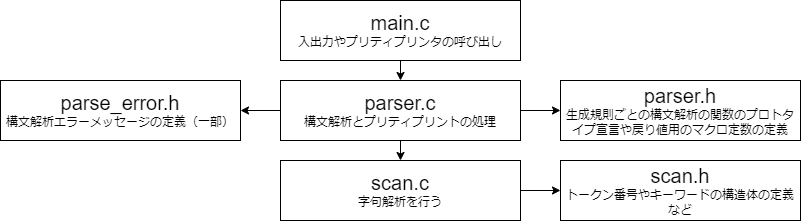
\includegraphics[width=\textwidth]{assets/module_02.png}
  \caption{課題2のモジュール構成図}
  \label{fig:module_graph}
\end{figure}

\subsection{各モジュールごとの構成}

\subsubsection{main.c}
init\_scan関数とend\_scan関数でファイルの開閉を行い,parse関数で構文解析とプリティプリントを行う.

\subsubsection{parser.c}
scan関数でトークンを取得してLL(1)構文木を作成して利用するのが短期間では困難だったため,結局断念して構文解析とプリティプリントを同時に行うようにした.

\subsubsection{scan.c}
字句解析を行い,得た文字列や数値はstring\_attrとnum\_attrに格納しておく.

\subsection{実装における外部仕様}
parse.cについてのみ触れる.

まず,変数を以下に示す.

\subsubsection{indent\_level}
\begin{description}
  \item[説明] インデントの深さを記憶する変数.0から始まる.
\end{description}

\subsubsection{br\_flag}
\begin{description}
  \item[説明] 改行が発生したかを記憶する変数.発生した場合は1,しない場合は0.pretty\_print関数が呼ばれると内部でフラグが0に設定される.
\end{description}

\subsubsection{iter\_flag}
\begin{description}
  \item[説明] 繰り返し文がどれだけの深さ発生しているかを記憶する変数.繰り返し文に入る度にインクリメントされ,breakで抜けるとデクリメントされる.
\end{description}

\subsubsection{formal\_arg\_flag}
\begin{description}
  \item[説明] 仮引数内を解析中かどうかを記憶する変数.1なら仮引数内,0なら仮引数外.
\end{description}

\subsubsection{empty\_stmt\_flag}
\begin{description}
  \item[説明] 空文があるかどうかを記憶する変数.1なら空文で,0なら空文でない.
\end{description}

次に関数について以下に示す.

\subsubsection{newline}
\begin{description}
  \item[機能] 改行を行い,br\_flagを1にする
  \item[引数] なし
  \item[戻り値] なし
\end{description}

\subsubsection{pretty\_print}
\begin{description}
  \item[機能] 各トークンについて適切なプリティプリントを行う
  \item[引数] なし
  \item[戻り値] なし
\end{description}

\subsubsection{parse}
\begin{description}
  \item[機能] 構文解析を開始し,プリティプリントも行う
  \item[引数] なし
  \item[戻り値] 構文解析に成功したら0,失敗したら-1
\end{description}

\subsubsection{parse\_○○}
\begin{description}
  \item[機能] 生成規則に対応した構文解析を再帰的に行う.また,都度プリティプリントを行う.
  \item[引数] なし
  \item[戻り値] 構文解析に成功したら0,失敗したら-1
\end{description}

\section{テスト情報}

\subsection{テストデータ}
\subsubsection{ブラックボックステスト}
ブラックボックステストには用意されていたテストデータを用いた.テストデータを以下に示す.
\begin{itemize}
  \item sample11.mpl
  \item sample011.mpl
  \item sample11p.mpl
  \item sample11pp.mpl
  \item sample12.mpl
  \item sample012.mpl
  \item sample12cr.mpl
  \item sample12crlf.mpl
  \item sample012eof.mpl
  \item sample12lf.mpl
  \item sample12lfcr.mpl
  \item sample012n.mpl
  \item sample012neof.mpl
  \item sample012s.mpl
  \item sample012seof.mpl
  \item sample13.mpl
  \item sample013.mpl
  \item sample14.mpl
  \item sample014.mpl
  \item sample014a.mpl
  \item sample014b.mpl
  \item sample14p.mpl
  \item sample15.mpl
  \item sample15a.mpl
  \item sample16.mpl
  \item sample17.mpl
  \item sample18.mpl
  \item sample19p.mpl
  \item sample2a.mpl
  \item sample02a.mpl
  \item sample21.mpl
  \item sample021.mpl
  \item sample22.mpl
  \item sample022.mpl
  \item sample23.mpl
  \item sample023.mpl
  \item sample24.mpl
  \item sample024.mpl
  \item sample24a.mpl
  \item sample25.mpl
  \item sample025.mpl
  \item sample025a.mpl
  \item sample25t.mpl
  \item sample26.mpl
  \item sample026.mpl
  \item sample26a.mpl
  \item sample27.mpl
  \item sample28p.mpl
  \item sample29p.mpl
\end{itemize}

\subsubsection{ホワイトボックステスト}
ブラックボックステストに用いたデータと同じものを用いた.

\subsection{テスト結果}
\subsubsection{ブラックボックステスト}
docker環境でのブラックボックステストの結果を図\ref{fig:black_box_test}に示す.
\begin{figure}[H]
  \centering
  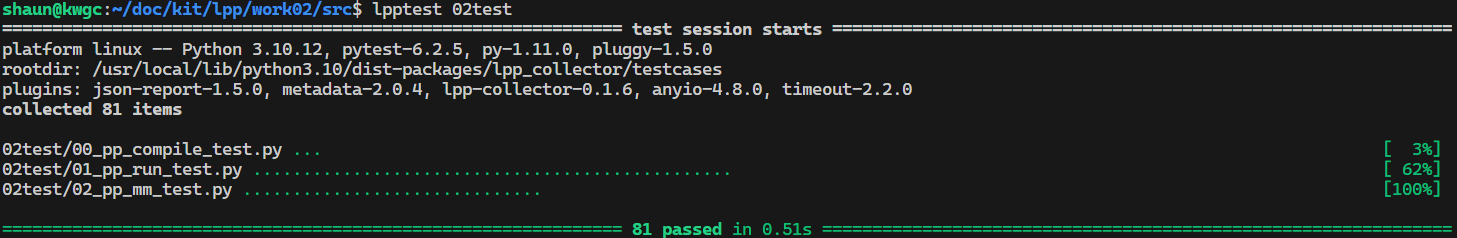
\includegraphics[width=\textwidth]{assets/black_box_test.png}
  \caption{ブラックボックステストの結果}
  \label{fig:black_box_test}
\end{figure}

\subsection{ホワイトボックステスト}
ホワイトボックステストの結果(主に実装を行ったparser.cについて)を図\ref{fig:white_box_test}に示す.
\begin{figure}[H]
  \centering
  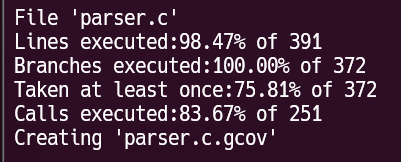
\includegraphics[width=\textwidth]{assets/white_box_test.png}
  \caption{ホワイトボックステストの結果}
  \label{fig:white_box_test}
\end{figure}

\subsection{テストデータの十分性}
ブラックボックステストでは生成規則についてのテストがほぼ全て含まれており,それらがパスしたことによりある程度の仕様を満たしていると考えられる.
また,ホワイトボックステストでは命令網羅率が$98.47\%$と高い数値を叩きだしており,コードの漏れが少ないと考えられる.

\section{課題のスケジュールと実際の進捗状況}
\subsection{事前計画}
\begin{table}[H]
  \centering
  \caption{課題2の事前計画}
  \begin{tabular}{cccp{7cm}}
    \hline
    開始日 & 終了日 & 予定工数(h) & 作業内容                                 \\ \hline
    1/7    & 1/9    & 4           & 資料を読んで仕様をまとめ,概略設計を行う \\
    1/8    & 1/12   & 10          & プログラムの作成                         \\
    1/8    & 1/12   & 4           & テスト工程                               \\
    1/10   & 1/12   & 4           & レポート作成                             \\
    \hline
  \end{tabular}
\end{table}

\subsection{実際の進捗状況}
\begin{table}[H]
  \centering
  \caption{課題2の事前計画}
  \begin{tabular}{cccp{7cm}}
    \hline
    開始日 & 終了日 & 工数(h) & 作業内容                                 \\ \hline
    1/7    & 1/9    & 4       & 資料を読んで仕様をまとめ,概略設計を行う \\
    1/8    & 1/23   & 20      & プログラムの作成                         \\
    1/8    & 1/23   & 5       & テスト工程                               \\
    1/18   & 1/23   & 3       & レポート作成                             \\
    \hline
  \end{tabular}
\end{table}

\subsection{当初の事前計画と実際の進捗との差の原因}
課題1がかなり遅れたため,課題2にも響いてしまい,本来の締め切りを超過している.
また,今回の課題に関して予定よりも工数がかかってしまった原因は,構文解析の結果から抽象構文木を作成して
プリティプリントを行おうとし,その実装と調査に時間がかかってしまったことが大きい.MPPLの生成規則から
構文木を作成して利用するのが短期間では困難だったため,結局断念して構文解析とプリティプリントを同時に行うようにした.

\end{document}